\documentclass[11pt,a4paper]{article}
\usepackage[T1]{fontenc}
\usepackage[utf8]{inputenc}
\usepackage[polish]{babel}
\usepackage[margin=2cm]{geometry}
\usepackage{graphicx}
\usepackage{amsmath}
\usepackage{booktabs}
\usepackage{listings}
\usepackage{xcolor}
\usepackage[hidelinks]{hyperref}

\lstset{
  language=C++,
  basicstyle=\ttfamily\scriptsize,
  breaklines=true,
  frame=single,
  tabsize=4,
  columns=fullflexible,
  keepspaces=true,
  backgroundcolor=\color{gray!8},
  extendedchars=true,
  literate={ą}{{\k{a}}}1 {ć}{{\'c}}1 {ę}{{\k{e}}}1 {ł}{{\l{}}}1 {ń}{{\'n}}1
           {ó}{{\'o}}1 {ś}{{\'s}}1 {ź}{{\'z}}1 {ż}{{\.z}}1 {Ł}{{\L{}}}1
}

% Zdjęcie z internetu: wstaw plik do img/, inaczej pusta ramka
\newcommand{\zdjecie}[2]{\IfFileExists{img/#1}%
  {\includegraphics[width=#2]{img/#1}}%
  {\fbox{\parbox[c][4cm][c]{#2}{\centering\small brak pliku img/\detokenize{#1}}}}}

\title{Symulacja pożaru Camp Fire (2018) w IGA-ADS}
\author{Rafał Szepieniec}
\date{\today}

\begin{document}
\maketitle

\section{Wybrany pożar: Camp Fire}

Camp Fire wybuchł 8 listopada 2018 r. ok.\ 6:25 w kanionie rzeki Feather koło Pulga
(hrabstwo Butte, Kalifornia). Przyczyną była awaria linii przesyłowej PG\&E.
Silny, suchy wiatr z północnego wschodu pchał ogień na południowy zachód.
W ciągu kilku godzin pożar przeszedł przez Concow i Magalię i dotarł do Paradise.
Ogień przeskakiwał kaniony dzięki żarowi niesionemu wiatrem.
Spłonęło ok.\ 620\,km$^2$ i ok.\ 18\,800 budynków, a zginęło 85 osób.
Był to najtragiczniejszy pożar w historii Kalifornii.

\begin{figure}[htbp]
\centering
\zdjecie{zdjecie_1.jpg}{0.48\textwidth}\hfill
\zdjecie{zdjecie_2.jpg}{0.48\textwidth}
\caption{Camp Fire (źródło: \dots).}
\end{figure}

Przebieg pożaru w czasie pochodzi z raportu NIST TN 2135 \cite{nist}: 2836 obserwacji ognia
z godziną i współrzędnymi GPS (rys.~\ref{fig:nist}).

\begin{figure}[htbp]
\centering
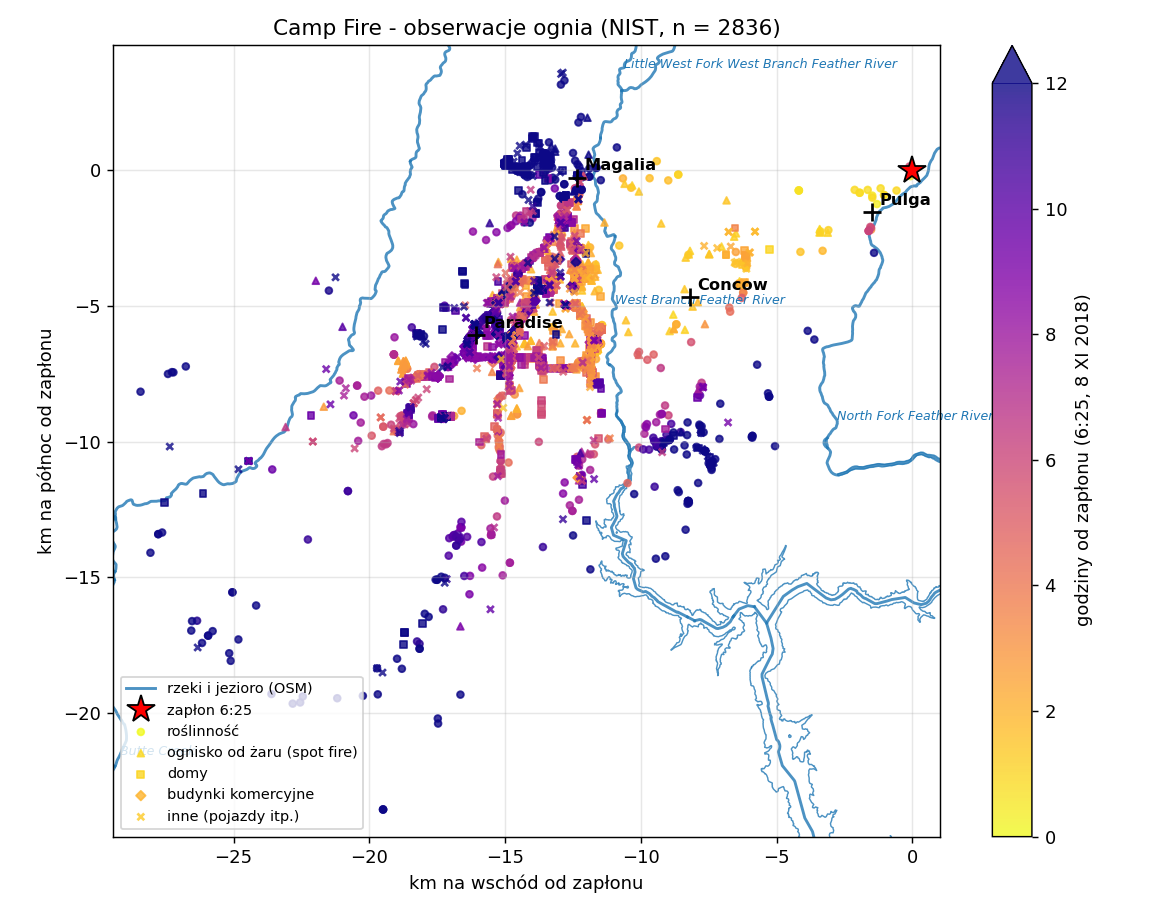
\includegraphics[width=0.75\textwidth]{img/nist_mapa.png}
\caption{Obserwacje ognia NIST, kolor oznacza liczbę godzin od zapłonu. Rzeki z OpenStreetMap.}
\label{fig:nist}
\end{figure}

\section{Model i dane}

Obszar modelu $[0,100]^2$ to kwadrat $30\times30$\,km wokół zapłonu (1 jednostka = 300\,m,
$x$ na wschód, $y$ na północ). Czas $t\in[0,10]$ odpowiada godzinom 6:25--11:25
(1 jednostka = 30\,min). Siatka ma $80\times80$ elementów, splajny są stopnia 2, a krok czasu
$\Delta t=10^{-3}$ (10\,000 kroków jawnej metody Eulera).

Równania z zajęć (temperatura $T$, paliwo $F$, wiatr $\mathbf b$):
\begin{align*}
\rho c_p \frac{\partial T}{\partial t} &= R_c - \rho c_w\, \mathbf b\cdot\nabla T
  + \nabla\cdot\big((\kappa + 4\sigma\varepsilon\delta_x T^3)\nabla T\big)
  + \xi (T_0 - T) + \frac{\sigma\varepsilon}{\delta_z}(T_0^4 - T^4),\\
\frac{\partial F}{\partial t} &= -\beta\, r F, \qquad
r = A_r T e^{-T_a/T}\ \text{gdy } T > T_{ig} \text{ i } F > F_{\min},\ \text{inaczej } 0,\\
R_c &= -I(x,y)\cdot 10^4 \rho c_h h_c \frac{M}{M_1}\, r .
\end{align*}

Dane wejściowe:
\begin{itemize}
\item paliwo: LANDFIRE 2016 FBFM40, stan sprzed pożaru \cite{landfire}, oraz rzeki z OpenStreetMap \cite{osm},
\item wiatr: stacja RAWS Jarbo Gap (JBGC1), pomiary co godzinę z archiwum IEM \cite{iem},
\item zapłon: pierwsza obserwacja NIST.
\end{itemize}
Skrypt \texttt{przygotuj\_model.py} przelicza te dane do pliku \texttt{camp\_fire\_data.hpp}
(mapa klas paliwa $201\times201$, tabela wiatru, punkt zapłonu).

\section{Zmiany w kodzie}

Zmienione pliki to \texttt{fire.hpp} i \texttt{fire.cpp} (pełny kod w dodatku~\ref{sec:kod}).
Wszystkie parametry i wagi paliwa są w strukturze \texttt{fire\_params}.
Można je zmieniać bez kompilacji, np.\ \texttt{fire 80 2 8 TU=0.6 cw=1.0}.

\lstinputlisting[firstline=55,lastline=104]{kod/fire.hpp}

\paragraph{Stan początkowy.} Gorący obszar (1500\,K w promieniu 0,75\,km, spadek do 300\,K
w promieniu 2,1\,km) w miejscu pierwszej obserwacji NIST.
\lstinputlisting[firstline=152,lastline=156]{kod/fire.hpp}

\paragraph{Mapa paliwa.} Waga klasy LANDFIRE w danym punkcie, z interpolacją dwuliniową
między węzłami siatki $201\times201$. W pasie 150\,m wzdłuż rzek brana jest mniejsza
z wag klasy i \texttt{river}.
\lstinputlisting[firstline=158,lastline=170]{kod/fire.hpp}

\paragraph{Wiatr.} Liniowa interpolacja w czasie pomiarów z Jarbo Gap. Dane są z jednej
stacji, więc wiatr jest taki sam w całym obszarze. Przelicznik to 0,85 jednostki modelu
na 1\,m/s.
\lstinputlisting[firstline=172,lastline=178]{kod/fire.hpp}

\paragraph{Prawa strona równania.} Wprowadziliśmy trzy zmiany względem wersji z zajęć:
\begin{itemize}
\item ciepło spalania jest mnożone przez $I = \texttt{heat}\cdot w(x,y)$, gdzie $w$ to waga klasy
  paliwa (\texttt{fuel\_heat = 1}), więc krzewy grzeją mocniej niż podszyt;
\item temperatura jest obcinana od dołu do 0, bo bez tego oscylacje splajnów przy zapłonie
  dają NaN w całym polu;
\item progi i współczynniki pochodzą z \texttt{fire\_params}.
\end{itemize}
\lstinputlisting[firstline=223,lastline=255]{kod/fire.hpp}

\paragraph{Szerokość frontu.} Przy stałych z zajęć front ognia jest węższy (ok.\ 0,3 jednostki)
niż element siatki (1,25). Ogień wtedy zatrzymuje się na liniach siatki: idzie wzdłuż osi albo
gaśnie. Dlatego pomnożyliśmy \texttt{rad} ($\delta_x$) i \texttt{loss} ($\delta_z$) przez 6,
a \texttt{heat} i $\beta$ (\texttt{burn}) podzieliliśmy przez 6. Spalanie w punkcie trwa
wtedy 6 razy dłużej, progi zapłonu i gaśnięcia się nie zmieniają, a front jest ok.\ 6 razy
szerszy. Dla mnożników 3 i 6 wyniki są zbliżone.

\section{Mapa paliwa}

\begin{table}[htbp]
\centering
\begin{tabular}{@{}llrrr@{}}
\toprule
Klasa & Opis & Waga & Obszar & Obserwacje NIST \\
\midrule
SH & krzewy (chaparral) & 1.00 & 8\,\% & 1\,\% \\
GS & trawy z krzewami & 1.00 & 12\,\% & 5\,\% \\
GR & trawy & 0.80 & 21\,\% & 5\,\% \\
TU & podszyt leśny & 0.50 & 29\,\% & 5\,\% \\
TL & ściółka leśna & 0.90 & 24\,\% & 45\,\% \\
urban & zabudowa & 0.90 & 3\,\% & 38\,\% \\
agri, rock, water & pola, skały, woda & 0.15, 0.05, 0 & 4\,\% & $<1$\,\% \\
river & pas przy rzece & 0.55 & 4\,\% & -- \\
\bottomrule
\end{tabular}
\caption{Wagi paliwa. Ostatnie kolumny: udział klasy w obszarze i w obserwacjach ognia NIST do 11:25.}
\end{table}

Wagi dobraliśmy, porównując wyniki symulacji z obserwacjami NIST. Podszyt (TU) zajmuje 29\,\%
obszaru, ale ma tylko 5\,\% obserwacji ognia, dlatego jego waga leży poniżej progu
samodzielnego palenia (ok.\ 0,55). Ogień przechodzi przez podszyt tylko wtedy, gdy obok palą
się trawy lub krzewy. Ściółka sosnowa (TL) na grzbiecie Paradise i zabudowa mają większość
obserwacji. Obserwacje NIST pochodzą jednak głównie z okolic domów i dróg.

\begin{figure}[htbp]
\centering
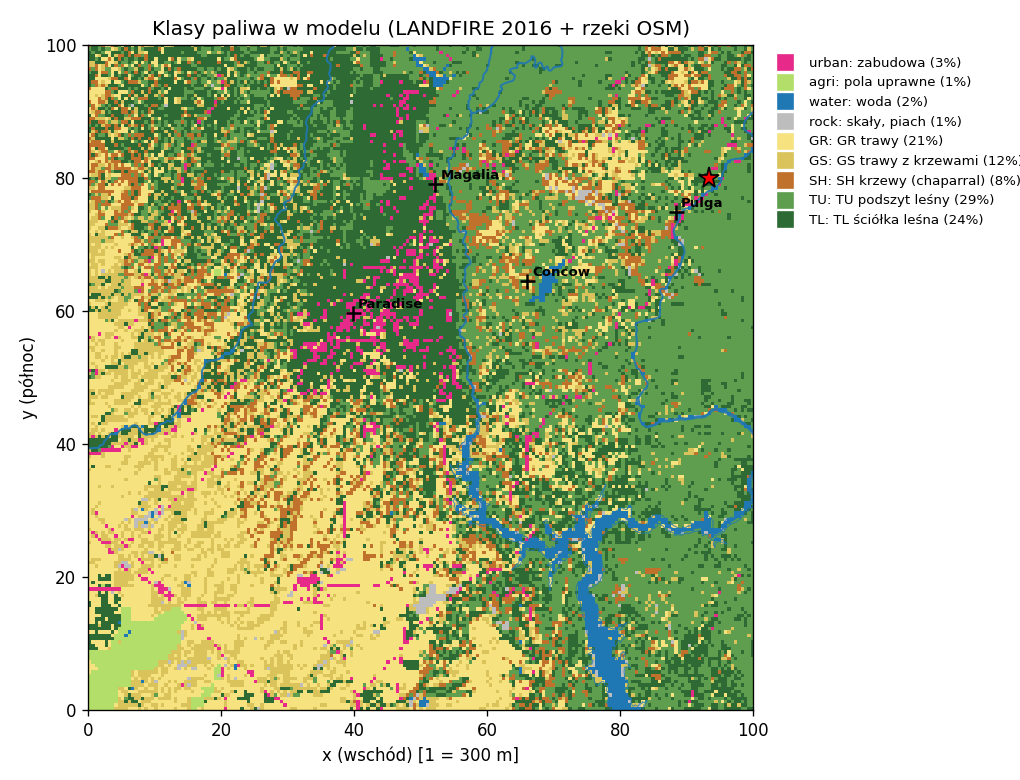
\includegraphics[width=0.56\textwidth]{img/model_klasy.png}\hfill
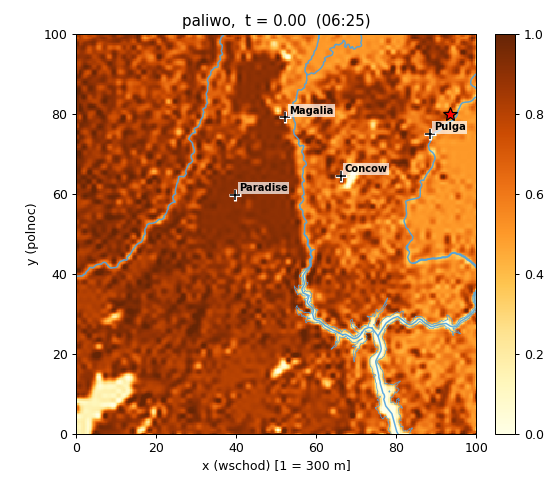
\includegraphics[width=0.42\textwidth]{img/fuel_0.png}
\caption{Klasy paliwa LANDFIRE w obszarze modelu (lewy) i \texttt{fuel\_init} po rzutowaniu na splajny (prawy).}
\end{figure}

\section{Stan początkowy}

\begin{figure}[htbp]
\centering
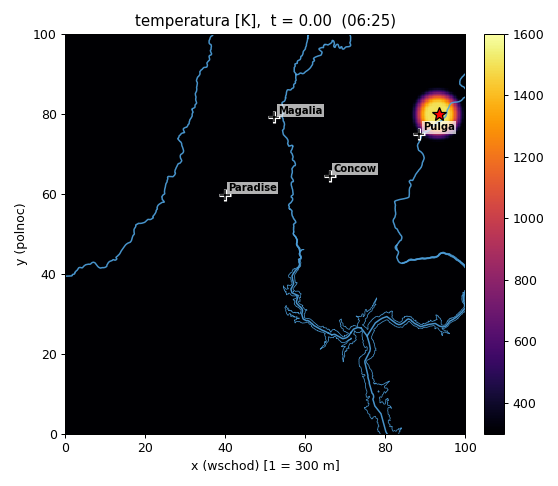
\includegraphics[width=0.5\textwidth]{img/fire_00000.png}
\caption{Temperatura w chwili $t=0$ (6:25). Gwiazdka oznacza zapłon.}
\end{figure}

\section{Wiatr}

\begin{table}[htbp]
\centering
\begin{tabular}{@{}lrrrrrrrrr@{}}
\toprule
Godzina & 5:13 & 6:13 & 7:13 & 8:13 & 9:13 & 10:13 & 11:13 & 12:13 & 13:13 \\
\midrule
Prędkość [m/s] & 13.4 & 8.1 & 6.3 & 2.7 & 6.3 & 8.1 & 6.3 & 7.2 & 5.4 \\
Skąd wieje [$^\circ$] & 42 & 33 & 33 & 14 & 33 & 37 & 29 & 31 & 38 \\
\bottomrule
\end{tabular}
\caption{Pomiary wiatru w Jarbo Gap, 8 XI 2018 (czas PST).}
\end{table}

Wiatr cały czas wieje z północnego wschodu. Najsilniejszy jest przed zapłonem, a ok.\ 8:00
na krótko słabnie.

\begin{figure}[htbp]
\centering
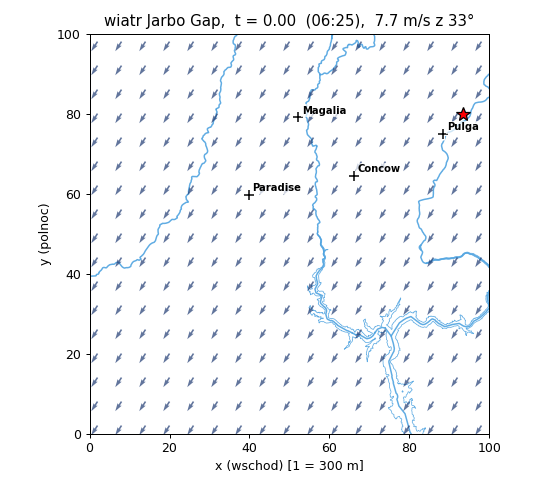
\includegraphics[width=0.24\textwidth]{img/wind_0_00.png}\hfill
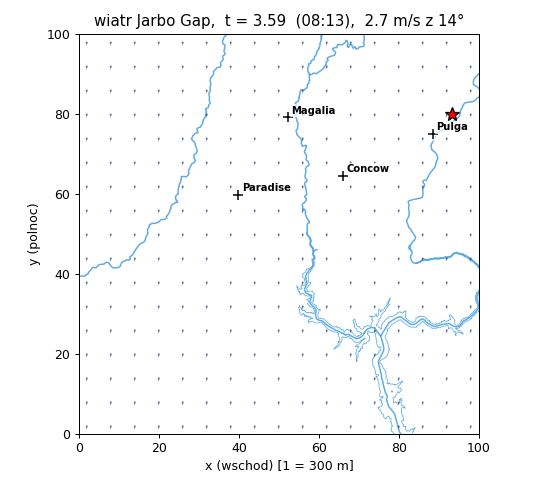
\includegraphics[width=0.24\textwidth]{img/wind_3_59.png}\hfill
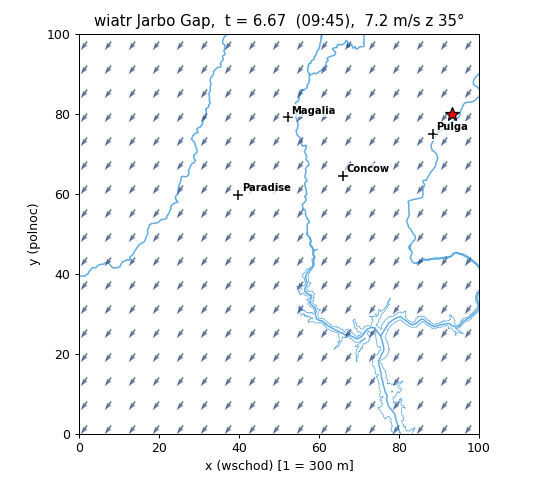
\includegraphics[width=0.24\textwidth]{img/wind_6_67.png}\hfill
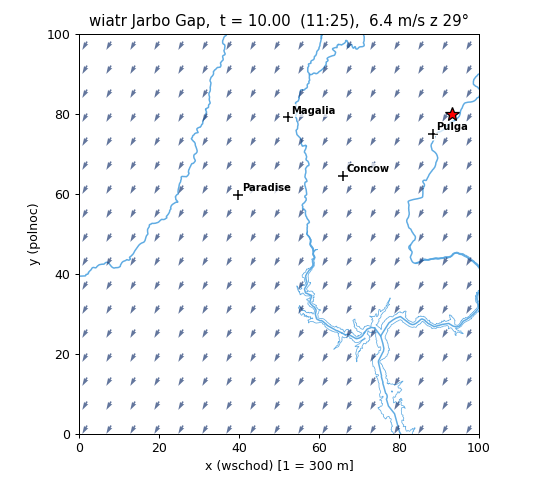
\includegraphics[width=0.24\textwidth]{img/wind_10_00.png}
\caption{Wiatr w modelu w chwilach $t = 0$, 3,6, 6,7 i 10 (6:25, 8:12, 9:45, 11:25).}
\end{figure}

\begin{figure}[htbp]
\centering
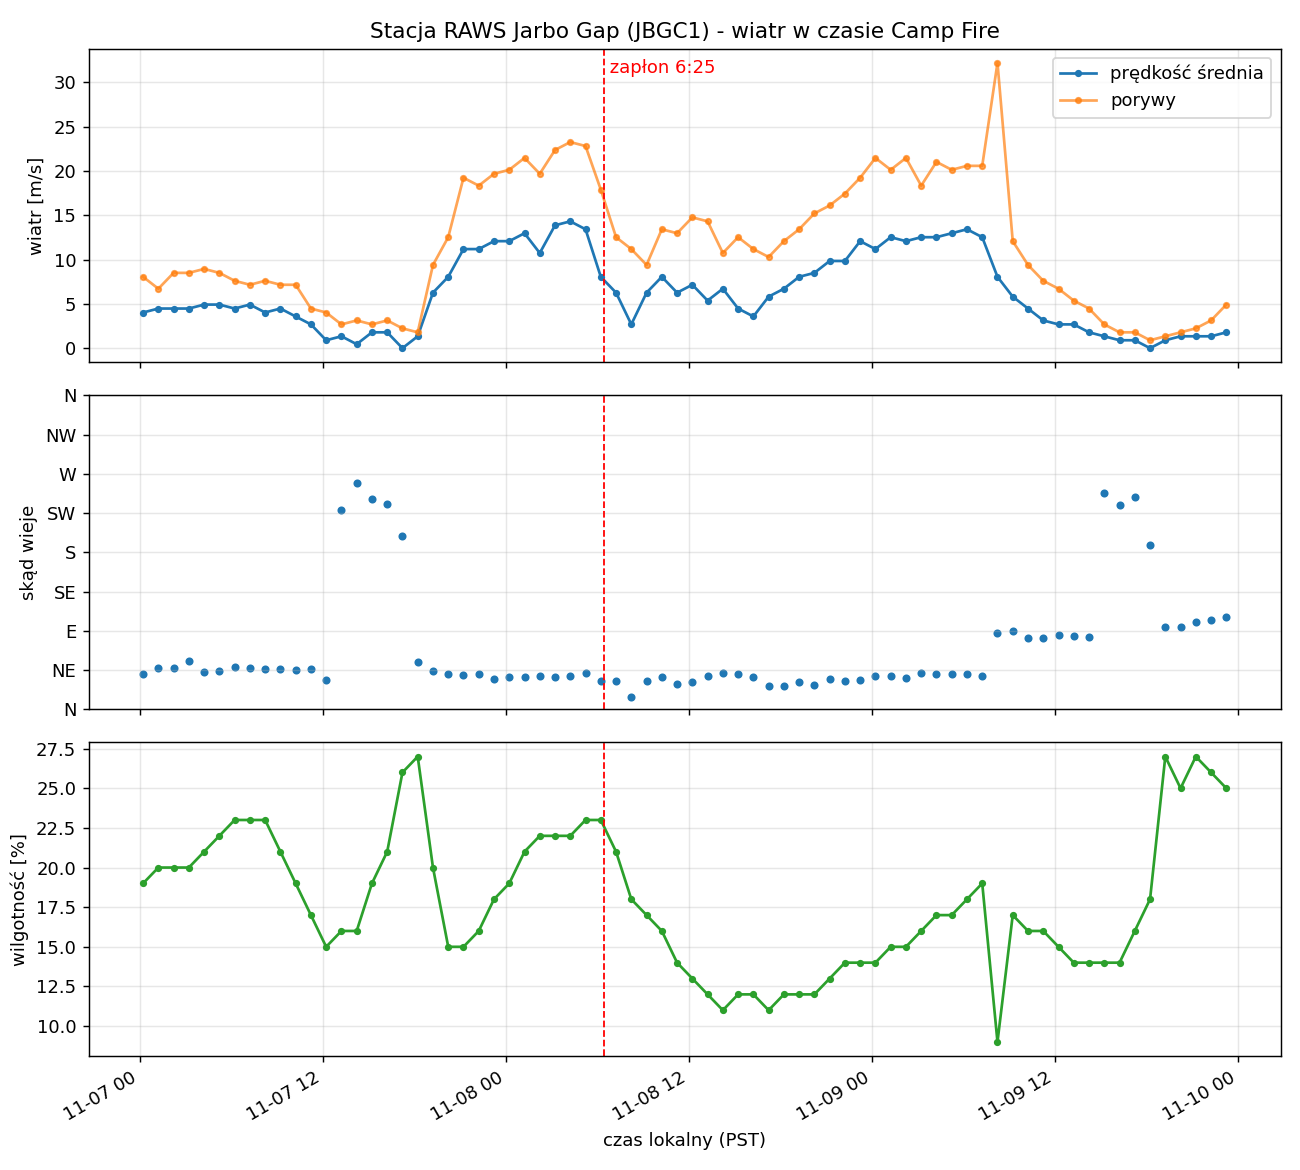
\includegraphics[width=0.7\textwidth]{img/wiatr_jarbo.png}
\caption{Pomiary ze stacji Jarbo Gap z 7--10 XI 2018.}
\end{figure}

\section{Animacje}

Animacje są w osobnych plikach GIF w katalogu \texttt{anim/}:
\begin{itemize}
\item \texttt{anim/fire.gif}: temperatura,
\item \texttt{anim/fuel.gif}: paliwo,
\item \texttt{anim/wind.gif}: wiatr,
\item \texttt{anim/pozar\_nist.gif}: rzeczywisty przebieg z obserwacji NIST.
\end{itemize}

\section{Kroki czasowe}

\begin{figure}[htbp]
\centering
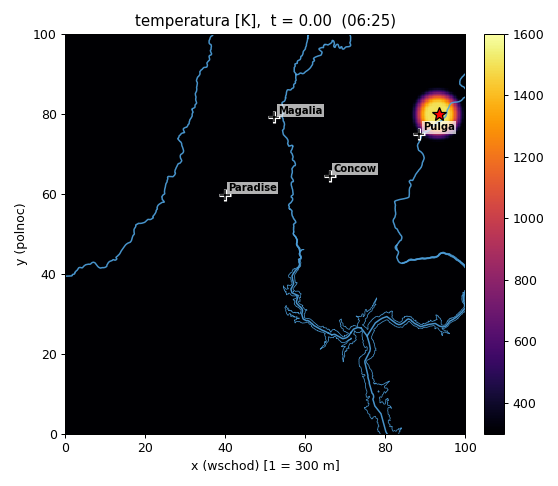
\includegraphics[width=0.24\textwidth]{img/fire_00000.png}\hfill
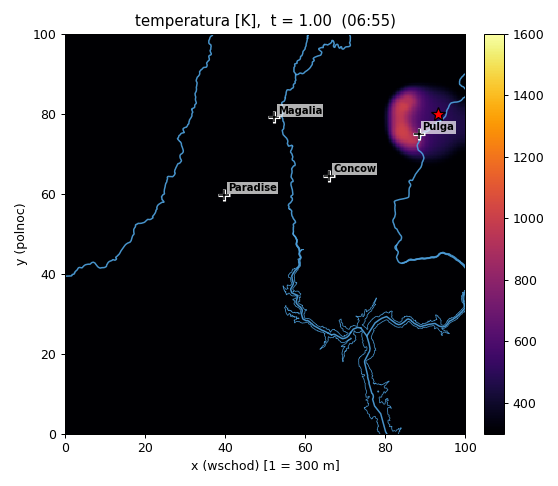
\includegraphics[width=0.24\textwidth]{img/fire_01000.png}\hfill
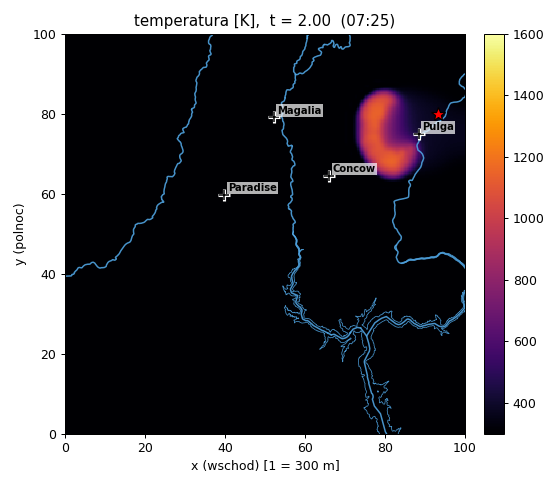
\includegraphics[width=0.24\textwidth]{img/fire_02000.png}\hfill
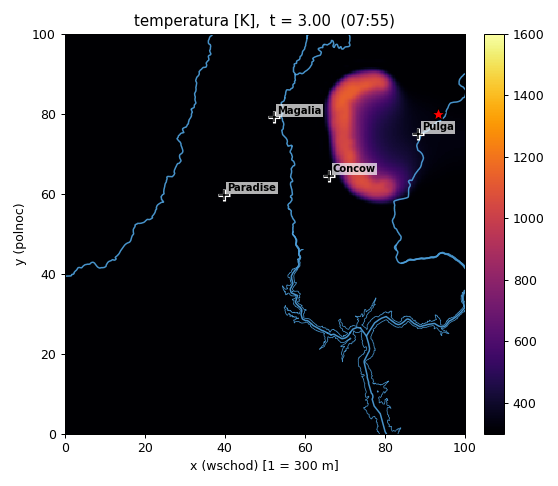
\includegraphics[width=0.24\textwidth]{img/fire_03000.png}\\[2mm]
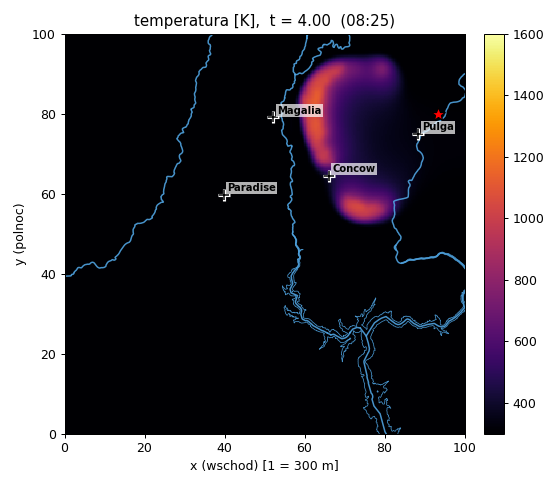
\includegraphics[width=0.24\textwidth]{img/fire_04000.png}\hfill
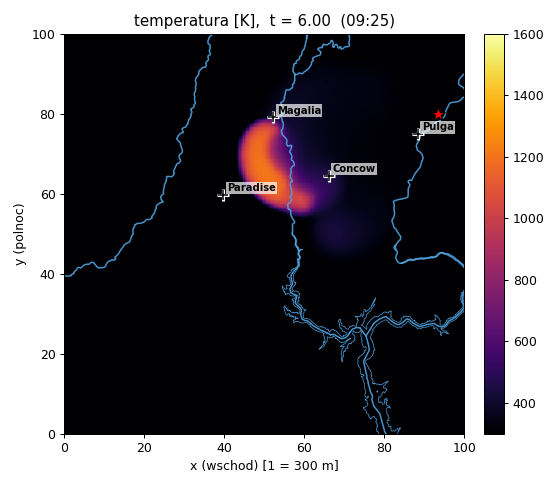
\includegraphics[width=0.24\textwidth]{img/fire_06000.png}\hfill
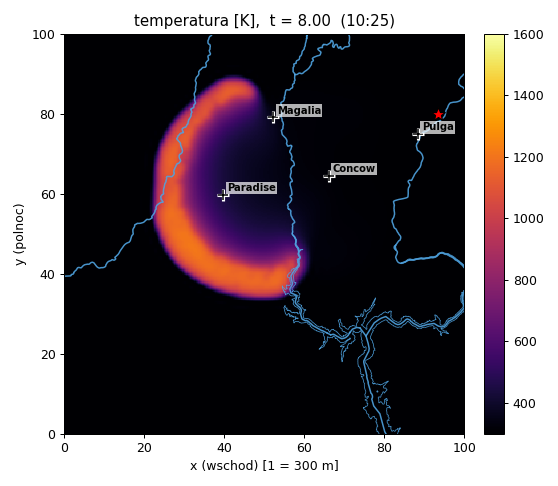
\includegraphics[width=0.24\textwidth]{img/fire_08000.png}\hfill
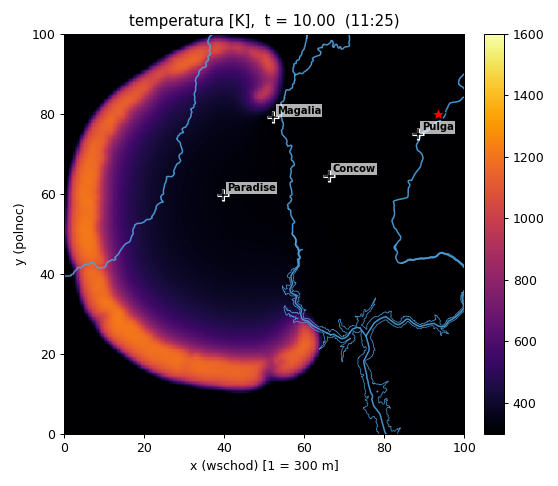
\includegraphics[width=0.24\textwidth]{img/fire_10000.png}
\caption{Temperatura co 30--60 min (kroki 0, 1000, 2000, 3000, 4000, 6000, 8000, 10\,000).}
\end{figure}

\begin{figure}[htbp]
\centering
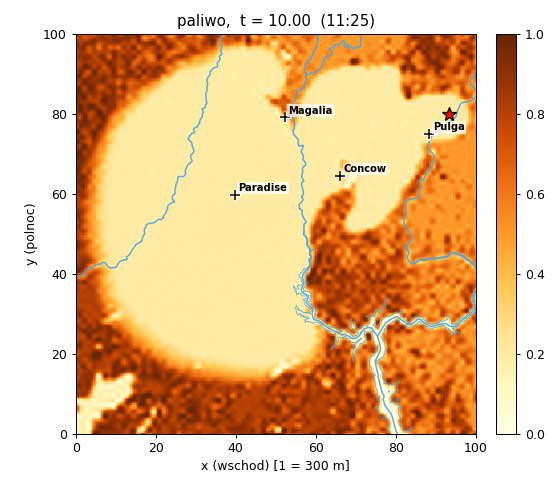
\includegraphics[width=0.45\textwidth]{img/fuel_10.png}
\caption{Paliwo o 11:25. Ciemne obszary spłonęły.}
\end{figure}

Ogień rusza z wiatrem na południowy zachód, wzdłuż korytarza traw i krzewów do Concow.
Ok.\ 8:25 front stoi na rzece West Branch, a potem przechodzi na grzbiet z Magalią
i Paradise. Podszyt na wschód i południe od zapłonu prawie się nie pali. Po 10:00 ogień
rozchodzi się po trawach na zachodzie.

\section{Porównanie z rzeczywistym pożarem}

\begin{figure}[htbp]
\centering
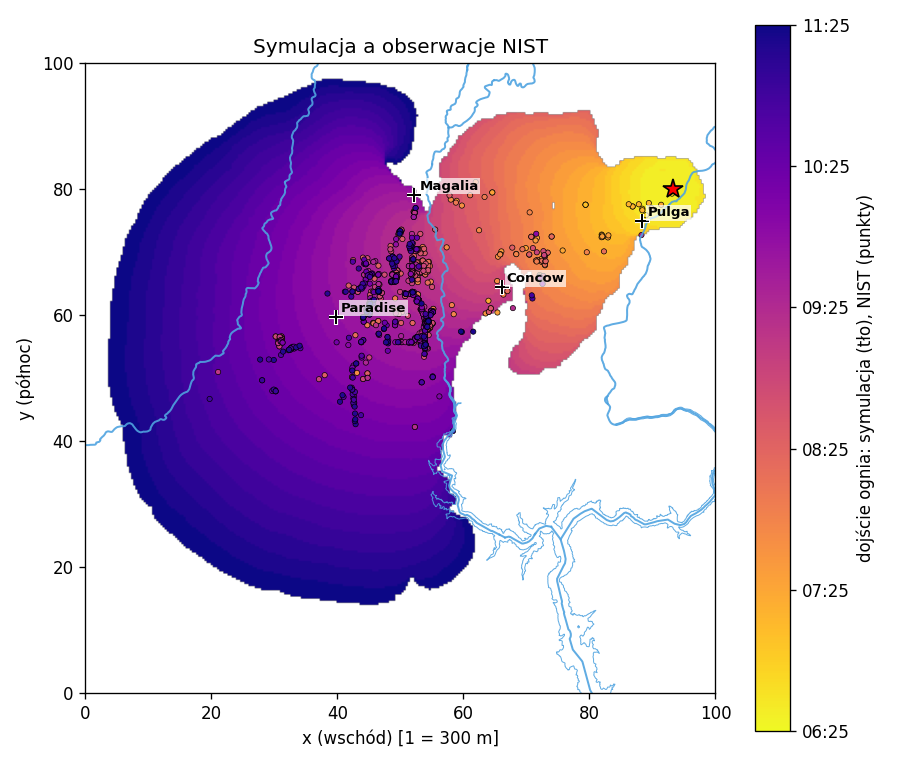
\includegraphics[width=0.65\textwidth]{img/porownanie_nist.png}
\caption{Czas dojścia ognia: tło pokazuje symulację, punkty obserwacje NIST (ta sama skala kolorów).}
\end{figure}

\begin{table}[htbp]
\centering
\begin{tabular}{@{}lr@{}}
\toprule
Obserwacje NIST do 11:25 objęte ogniem w symulacji & 99,7\,\% \\
\dots{} najpóźniej 30 min po obserwacji & 67,0\,\% \\
Mediana opóźnienia (symulacja $-$ NIST) & $+2$ min \\
Spalona część palnego obszaru & 48,6\,\% \\
\bottomrule
\end{tabular}
\quad
\begin{tabular}{@{}lcc@{}}
\toprule
Miejscowość & Symulacja & NIST \\
\midrule
Pulga & 6:33 & 6:46 \\
Concow & 8:10 & 7:24 \\
Magalia & 8:55 & 8:01 \\
Paradise & 9:40 & 10:46 \\
\bottomrule
\end{tabular}
\caption{Zgodność z NIST (lewa tabela) i pierwsze dojście ognia w promieniu 1,2\,km od miejscowości (prawa tabela).}
\end{table}

\begin{table}[htbp]
\centering
\begin{tabular}{@{}lccc@{}}
\toprule
Waga TU & Spalone & Objęte obserwacje NIST & Mediana opóźnienia \\
\midrule
0.4 & 1,1\,\% & 1,6\,\% & ogień gaśnie przy zapłonie \\
0.5 & 48,6\,\% & 99,7\,\% & $+2$ min \\
0.6 & 78,9\,\% & 100\,\% & $-25$ min \\
\bottomrule
\end{tabular}
\caption{Wpływ wagi podszytu leśnego (TU).}
\end{table}

Kierunek i tempo pożaru zgadzają się z obserwacjami: mediana różnicy czasu dojścia ognia
wynosi kilka minut, a symulacja obejmuje prawie wszystkie punkty NIST. Główne różnice:
\begin{itemize}
\item do Concow i Magalii ogień dochodzi ok.\ 45--55 min za późno, bo model nie ma żaru
  niesionego wiatrem, dzięki któremu ogień przeskakiwał kaniony;
\item po 10:00 ogień rozchodzi się prawie kołowo po trawach, a spalony obszar jest
  większy niż w rzeczywistości;
\item model nie uwzględnia rzeźby terenu, a wiatr jest z jednej stacji, więc taki sam w całym obszarze.
\end{itemize}

\begin{thebibliography}{9}
\bibitem{nist} A. Maranghides i in., \emph{A Case Study of the Camp Fire -- Fire Progression
  Timeline}, NIST Technical Note 2135, 2021. Dane: \url{https://data.nist.gov/od/id/mds2-2954}
\bibitem{landfire} LANDFIRE 2016 Remap, Fire Behavior Fuel Model 40, USGS/USFS,
  \url{https://www.landfire.gov}
\bibitem{osm} \copyright{} współtwórcy OpenStreetMap (ODbL), \url{https://www.openstreetmap.org/copyright}
\bibitem{iem} Iowa Environmental Mesonet, stacja JBGC1, \url{https://mesonet.agron.iastate.edu}
\bibitem{ads} M. Łoś, IGA-ADS, \url{https://github.com/marcinlos/iga-ads}
\end{thebibliography}

\appendix
\section{Kod}
\label{sec:kod}

\subsection*{fire.hpp}
\lstinputlisting{kod/fire.hpp}

\subsection*{fire.cpp}
\lstinputlisting{kod/fire.cpp}

\end{document}
